% Chapter Template

\chapter{Results and Discussion}

\label{Chapter6:Results}

%----------------------------------------------------------------------------------------
% Transfer learning
% effect of loss function
% effect of camera intrinsic 
% effect of Hyper parameter
% Effect of recreating holes.. 
 
 
%----------------------------------------------------------------------------------------

In this section we have discussed three specific category to answer the three specfic question asking in the section \ref{Chapeter1:Topic_Description} 

% Please add the following required packages to your document preamble:
% \usepackage{multirow}
\begin{table}[h]
\begin{tabular}{p{0.05\linewidth}p{0.3\linewidth}p{0.1\linewidth}p{0.1\linewidth}p{0.1\linewidth}p{0.1\linewidth}p{0.1\linewidth}}
\hline
\textbf{\#} & \textbf{Model} & \multicolumn{3}{l}{\textbf{Accuracy}} & \multicolumn{2}{l}{\textbf{Error}} \\ \cline{3-7} 
                    &                        & a1       & a2       & a3      & rms         & log\_10      \\ \hline
\multicolumn{7}{l}{\texttt{Influence of Structural Characteristics}}                                            \\ \hline
\textbf{E1}                  &  \textbf{A1}               &          &          &         &             &              \\ \hline
\textbf{E2}                  & \textbf{A2}                  &          &          &         &             &              \\ \hline
\multicolumn{7}{l}{\texttt{Holes Regenration}}                                                                   \\ \hline
\textbf{E3}                  & \textbf{A2\_NoHoles}            & 0.98   & 0.98   & 0.98  & 0.10       & 0.18        \\ \hline
\textbf{E4}                  & \textbf{A2\_Holes}              & 0.39   & 0.58   & 0.65  & 0.27      & 1.70       \\ \hline
\multicolumn{7}{l}{\texttt{Infuence Of Transfer Learning}}                                                       \\ \hline
\textbf{E5}                  & \textbf{A2\_Holes}              & 0.39   & 0.58   & 0.65  & 0.27      & 1.70       \\ \hline
\textbf{E6}                  & \textbf{A2\_Holes} (Retrained) & 0.33   & 0.55   & 0.63  & 0.34      & 1.78       \\ \hline
\end{tabular}

\caption{This table list all the depth estimation experiment on Structure dataset. These experiments are grouped in to 3 catogories.}
\end{table}

\section{Influence of Structural Characteristics}
\label{Chapter6:Influence_Structural_Char}
In this section we have investigated the Influence of Structural Characteristics of a pre-trained network.  As discribed in the section \ref{Chapter5:Methodology} we designed \textbf{A1} a simple U-Net to test against a pre-trained network by ImageNet with DenseNet configuration \textbf{A2}. 
 
 
 
 
 
 
 \section{Hole Regeneration Method}
 \label{Chapter6:Hole_Regeneration}
In order to have a holes recreated we mapped all the dead value or no pixel region as zero pixel as discribed in section \ref{Chapter4:Dataset}. We tested \textbf{A2\_Holes} against the \textbf{A2\_NoHoles}.

As we see in Fig \ref{fig:results_S2}, we compare \textbf{E3} and \textbf{E4} fotr  





\begin{figure} 
\settoheight{\tempdima}{\includegraphics[width=.32\linewidth]{example-image-a}}%
\centering\begin{tabular}{@{}c@{ }c@{ }c@{ }c@{}}
&\textbf{RGB} & \textbf{Truth} & \textbf{Predticted} \\
\rowname{E3 $A2\_NoHoles$}&
\includegraphics[width=.3\linewidth]{Figures/results/s2_NoHoles/0RAW_RGB.png}&
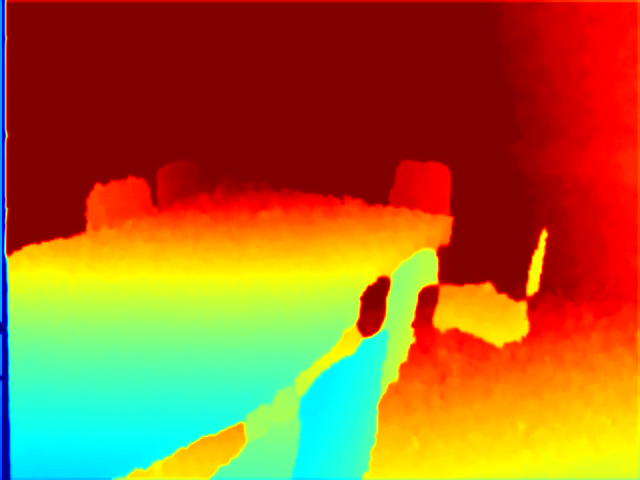
\includegraphics[width=.3\linewidth]{Figures/results/s2_NoHoles/0Truth.png}&
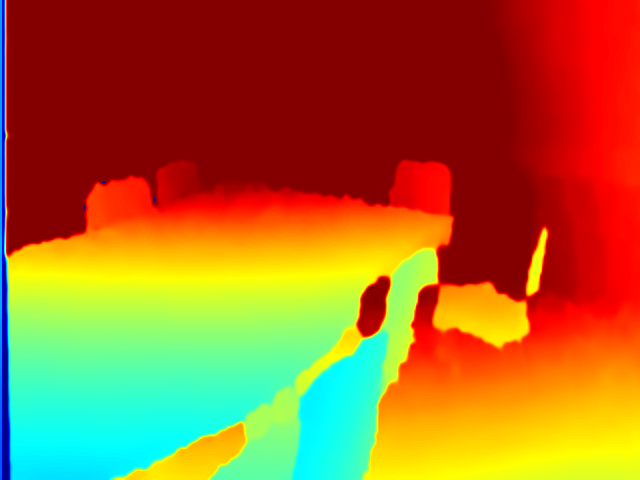
\includegraphics[width=.3\linewidth]{Figures/results/s2_NoHoles/0Predicted.png}\\[-1ex]
&\mycaption{} & \mycaption{} & \mycaption{} \\
\rowname{E3 $A2\_NoHoles$}&
\includegraphics[width=.3\linewidth]{Figures/results/s2_NoHoles/1RAW_RGB.png}&
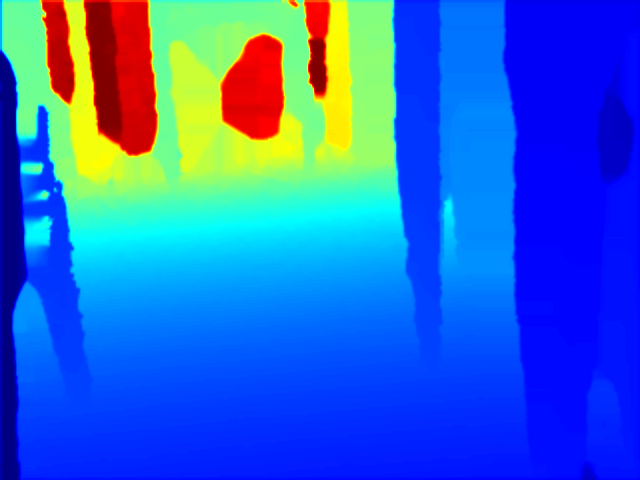
\includegraphics[width=.3\linewidth]{Figures/results/s2_NoHoles/1Truth.png}&
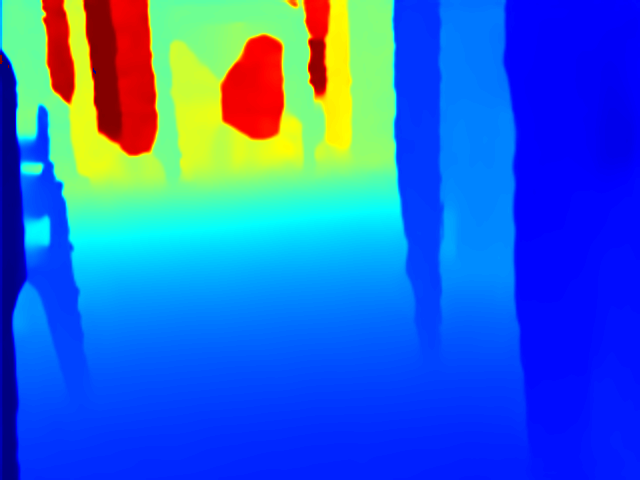
\includegraphics[width=.3\linewidth]{Figures/results/s2_NoHoles/1Predicted.png}\\[-1ex]
&\mycaption{} & \mycaption{} & \mycaption{} \\
\rowname{E3 $A2\_NoHoles$}&
\includegraphics[width=.3\linewidth]{Figures/results/s2_NoHoles/2RAW_RGB.png}&
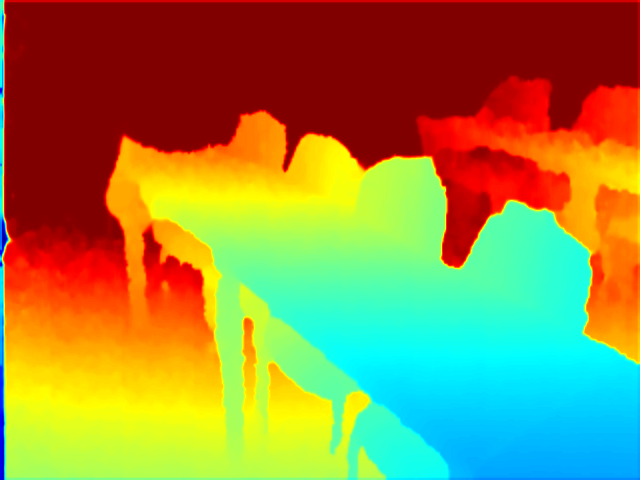
\includegraphics[width=.3\linewidth]{Figures/results/s2_NoHoles/2Truth.png}&
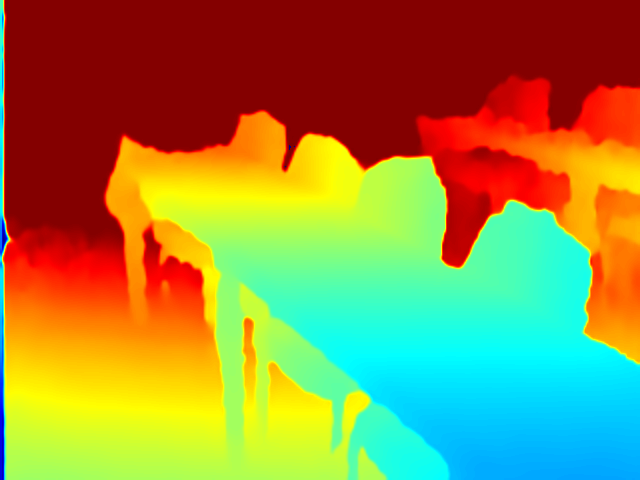
\includegraphics[width=.3\linewidth]{Figures/results/s2_NoHoles/2Predicted.png}\\[-1ex]
&\mycaption{} & \mycaption{} & \mycaption{} \\
\rowname{E4 $A2\_Holes$}&
\includegraphics[width=.3\linewidth]{Figures/results/s2_Holes/0RAW_RGB.png}&
\includegraphics[width=.3\linewidth]{Figures/results/s2_Holes/0Truth.png}&
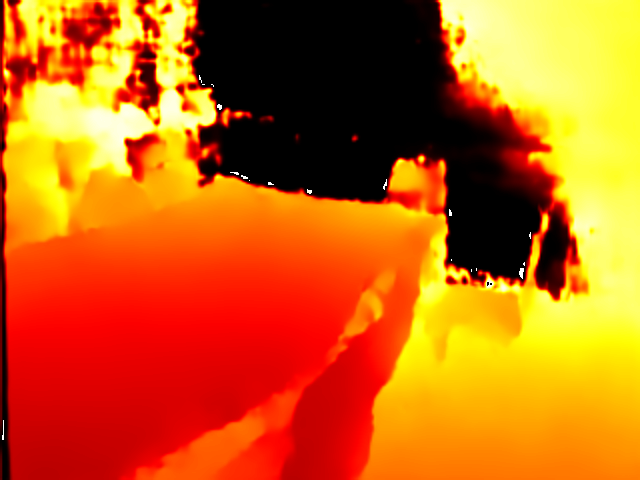
\includegraphics[width=.3\linewidth]{Figures/results/s2_Holes/0Predicted.png}\\[-1ex]
&\mycaption{} & \mycaption{} & \mycaption{} \\
\rowname{E4 $A2\_Holes$}&
\includegraphics[width=.3\linewidth]{Figures/results/s2_Holes/1RAW_RGB.png}&
\includegraphics[width=.3\linewidth]{Figures/results/s2_Holes/1Truth.png}&
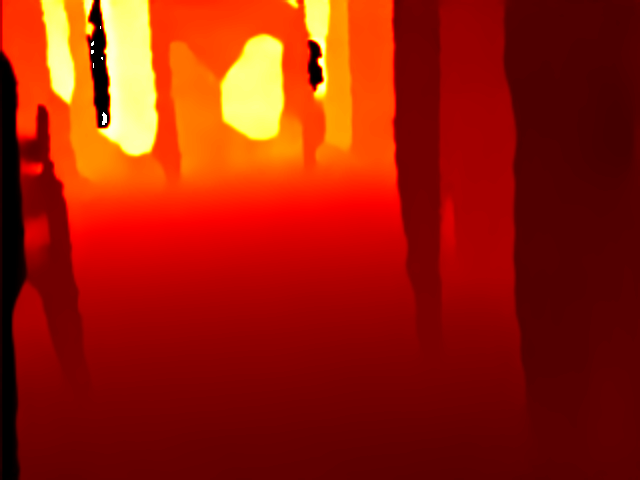
\includegraphics[width=.3\linewidth]{Figures/results/s2_Holes/1Predicted.png}\\[-1ex]
&\mycaption{} & \mycaption{} & \mycaption{} \\
\rowname{E4 $A2\_Holes$}&
\includegraphics[width=.3\linewidth]{Figures/results/s2_Holes/2RAW_RGB.png}&
\includegraphics[width=.3\linewidth]{Figures/results/s2_Holes/2Truth.png}&
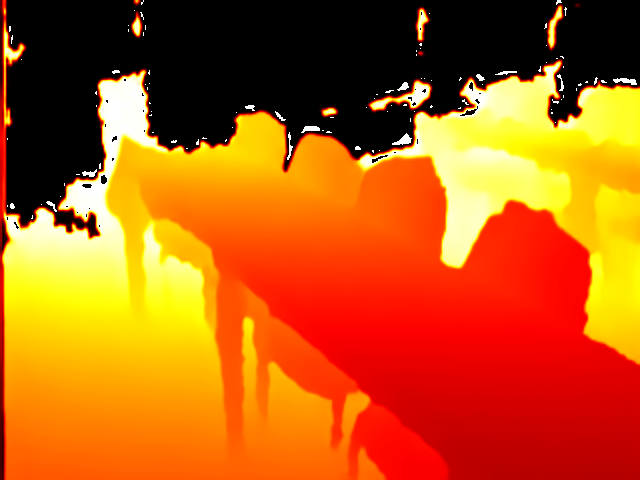
\includegraphics[width=.3\linewidth]{Figures/results/s2_Holes/2Predicted.png}\\[-1ex]
&\mycaption{} & \mycaption{} & \mycaption{} \\
\end{tabular}
\caption{\textbf{Investigation on hole regeneration method:} All the \textbf{E3} methods are in different  }%
\label{fig:results_S2}
\end{figure}




 \section{Infuence Of Transfer Learning}
 
 
 \begin{figure}
\settoheight{\tempdima}{\includegraphics[width=.32\linewidth]{example-image-a}}%
\centering\begin{tabular}{@{}c@{ }c@{ }c@{ }c@{}}
&\textbf{RGB} & \textbf{Truth} & \textbf{Predticted} \\
\rowname{E4 $A2\_Holes$}&
\includegraphics[width=.3\linewidth]{Figures/results/s2_Holes/0RAW_RGB.png}&
\includegraphics[width=.3\linewidth]{Figures/results/s2_Holes/0Truth.png}&
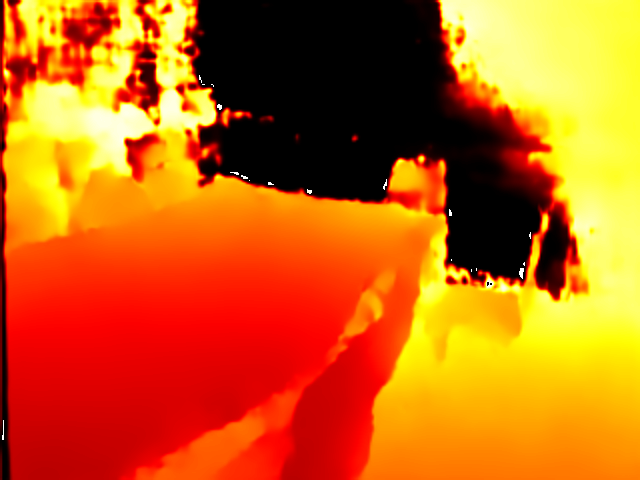
\includegraphics[width=.3\linewidth]{Figures/results/s2_Holes/0Predicted.png}\\[-1ex]
&\mycaption{} & \mycaption{} & \mycaption{} \\
\rowname{E4 $A2\_Holes$}&
\includegraphics[width=.3\linewidth]{Figures/results/s2_Holes/1RAW_RGB.png}&
\includegraphics[width=.3\linewidth]{Figures/results/s2_Holes/1Truth.png}&
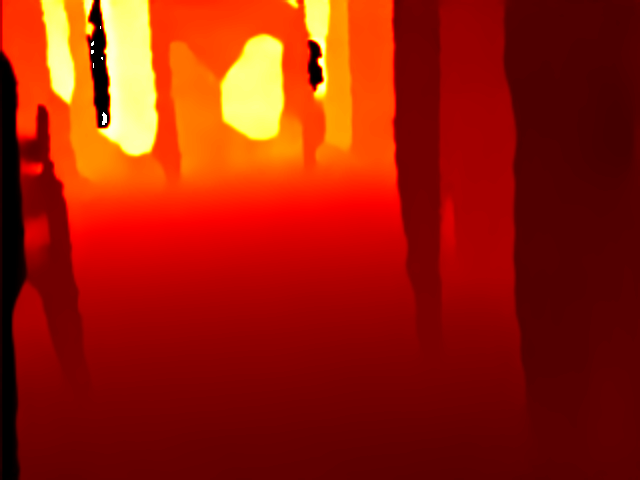
\includegraphics[width=.3\linewidth]{Figures/results/s2_Holes/1Predicted.png}\\[-1ex]
&\mycaption{} & \mycaption{} & \mycaption{} \\
\rowname{E4 $A2\_Holes$}&
\includegraphics[width=.3\linewidth]{Figures/results/s2_Holes/2RAW_RGB.png}&
\includegraphics[width=.3\linewidth]{Figures/results/s2_Holes/2Truth.png}&
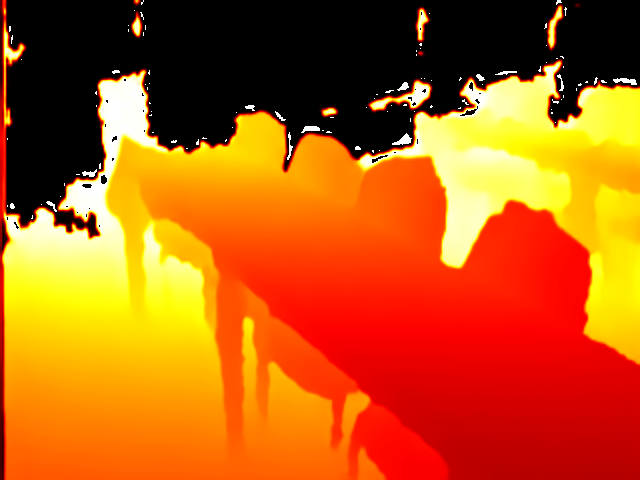
\includegraphics[width=.3\linewidth]{Figures/results/s2_Holes/2Predicted.png}\\[-1ex]
&\mycaption{} & \mycaption{} & \mycaption{} \\
\rowname{E3 $A2\_NoHoles$}&
\includegraphics[width=.3\linewidth]{Figures/results/s3_noNyu/0RAW_RGB.png}&
\includegraphics[width=.3\linewidth]{Figures/results/s3_noNyu/0Truth.png}&
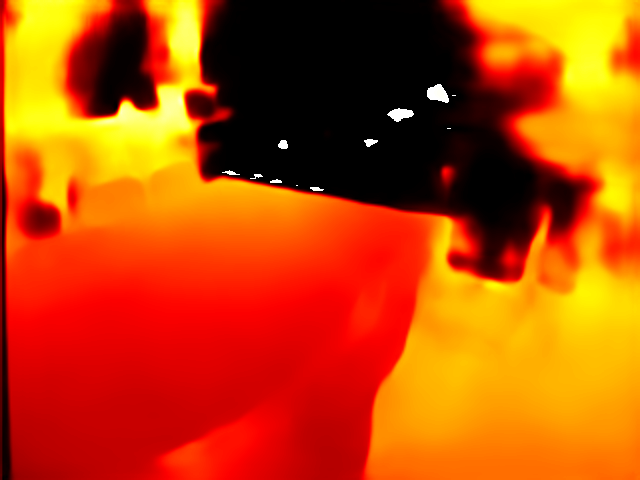
\includegraphics[width=.3\linewidth]{Figures/results/s3_noNyu/0Predicted.png}\\[-1ex]
&\mycaption{} & \mycaption{} & \mycaption{} \\
\rowname{E3 $A2\_NoHoles$}&
\includegraphics[width=.3\linewidth]{Figures/results/s3_noNyu/1RAW_RGB.png}&
\includegraphics[width=.3\linewidth]{Figures/results/s3_noNyu/1Truth.png}&
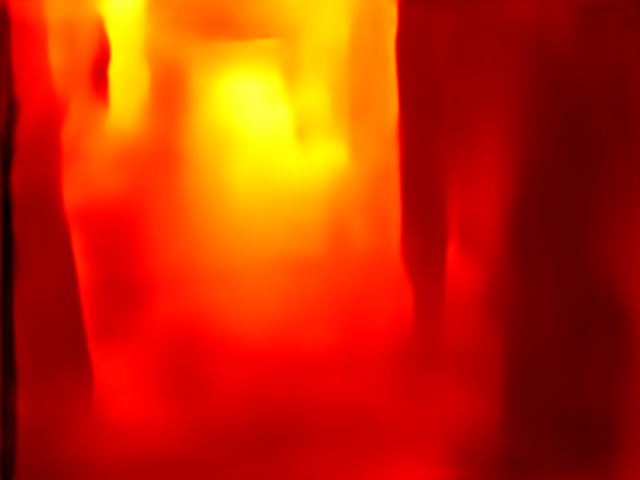
\includegraphics[width=.3\linewidth]{Figures/results/s3_noNyu/1Predicted.png}\\[-1ex]
&\mycaption{} & \mycaption{} & \mycaption{} \\
\rowname{E3 $A2\_NoHoles$}&
\includegraphics[width=.3\linewidth]{Figures/results/s3_noNyu/2RAW_RGB.png}&
\includegraphics[width=.3\linewidth]{Figures/results/s3_noNyu/2Truth.png}&
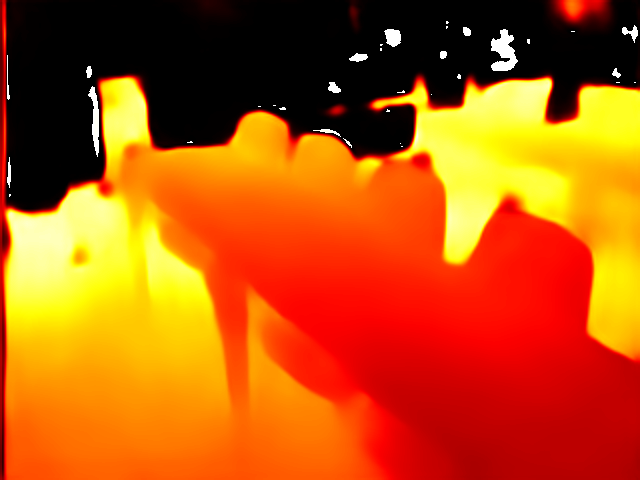
\includegraphics[width=.3\linewidth]{Figures/results/s3_noNyu/2Predicted.png}\\[-1ex]
&\mycaption{} & \mycaption{} & \mycaption{} \\
\end{tabular}
\caption{\textbf{Investigation on hole regeneration method:} All the \textbf{E3} methods are in different  }%
\label{figure1}
\end{figure}


 
 
 
 \label{Chapter6:Transfer_Learning}
In order to have a holes recreated we mapped all the dead value or no pixel region as zero pixel as described in section \ref{Chapter4:Dataset}. We tested \ this against the 